\section{Top-k Trace Alignment}\label{sec:topk}
{\color{green}[Fabrizio] Trace alignments algorithms provide as output a single alignment. This is not very convenient in practice because a rich feedback should provide different possibilities. This is even more important when the Petri Net we are considering is stochastic and the different model traces have different probabilities.}
%\texttt{\color{red}[TODO: introduction, motivation, and why it is useful to run it as a $k$-best search]}
%\resizeableyellownote{3}{3}{
%	Assuming that Rafael writes the definition of his ranking function, that can be expressed as $r(\tau^*,\tau)=d(\tau^*,\tau)w_\tau$ for a query trace $\tau^*$ and a trace $\tau\in\mathcal{W}_p^n(P)$
%}

In particular, we want to exploit the well-known \textit{k}-nearest neighbour problem for providing this desired result. Such problem can be formalized as follows:
\begin{definition}[$k$-Nearest Neighbour]
	Given a set of vectors  $\mathcal{X}\subseteq \mathbb{R}^d$ within a $d$-dimensional Euclidean space and a query vector $q\in\mathbb{R}^d$, the $k$-nearest neighbour algorithm returns a subset $K\subseteq\mathcal{X}$ of $k$ elements minimizing the distance from $v$:
	$$knn_\delta(k,q,\mathcal{X})=\begin{cases}
	\emptyset& k \leq 0\\
	\{c\}\cup knn(k-1,q,\mathcal{X}\backslash\{c\}) & k> 0 \Rightarrow c:={\arg\min}_{x\in\mathcal{X}}\delta(x,q)\\
	\end{cases}$$
	where $\delta$ is a distance measure between the vectors.
\end{definition}

\subsection{Exact $k$-probabilistic Traces Alignment Problem}\label{subsec:exbkptap}
%\texttt{\color{red}[TODO: the introduction of this section depends on how we want to formulate the problem. I suddenly start with the definition of the k-Nearest Neighbour, but I am aware that we need to provide first a bit of context]}



In order to reduce the exact probabilistic trace alignment problem to the \textit{k}-nearest neighbour, we can first map each weighted trace  $\braket{\tau,w_\tau}\in\mathcal{W}_p^n(P)$ that we need to align with $\tau^*$ as a point $\tau\overset{\mu_{\tau^*}}{\mapsto}(w_\tau,\; s_d(\tau,\tau^*))$ in the 2-dimensional similarity/probability space of coordinates $(p,s)$, so that the trace finding problem reduces to find a data point maximising the product $p\cdot s\equiv w_\tau\cdot s_d(\tau,\tau^*)$ (Figure \ref{fig:spp}).

\begin{table}[!t]
\centering
\caption{Expected ranking of the paths from Example \ref{ex:withpaths} with the trace $\tau^*=\textup{caba}$. The cost function is the one from \cite{LeoniM17} and its normalized similarity score has $c=5$.}\label{tab:expected}
\begin{tabular}{lc|ll|cl}
	\toprule
	
	\multirow{2}{*}{$\tau$} &
	\multirow{2}{*}{$d(\tau,\tau^*)$} &
	\multicolumn{2}{c|}{$\mu_{\tau^*}$} &
	 \multirow{2}{*}{$\approx s_d(\tau,\tau^*)\cdot w_\tau$} & \multirow{2}{*}{\textit{expected ranking}}\\
	
	\cline{3-4} &&  $\langle w_\tau$ &  $,\,s_d(\tau,\tau^*)\rangle $ &&\\
	
	\midrule
	{a}  & $3$ & $0.4$ & $\;\; 0.6250$  & $0.2500$ & \textbf{1}\\
	{aa}  & $2$ & $0.2$ & $\;\; 0.7142$ & $0.1428$ & \textbf{2}\\
	{aaa}  & $2$ & $0.1$ & $\;\; 0.7142$ & $0.0714$ & \textbf{3}\\
	{ca}  & $2$ & $0.07$ & $\;\; 0.7142$ & $0.0500$ & \textbf{4}\\
	{cb}  & $2$ & $0.06$ & $\;\; 0.7142$ & $0.0428$ & \textbf{5}\\
	{aaaa}  & $3$ & $0.05$ & $\;\; 0.7142$ & $0.0357$ & \textbf{6}\\
	{caa}  & $1$ & $0.035$ & $\;\; 0.8333$ & $0.0292$ &  \textbf{7}\\
	{caaa}  & $1$  & $0.0175$ & $\;\; 0.8333$ & $0.0145$ & \textbf{8}\\
	\bottomrule
\end{tabular}
\end{table}
\begin{example}\label{ex:rankingTaus}
Table \ref{tab:expected} represents the expected exact alignment raking of all the weighted traces $\braket{\tau,w_\tau}\in\mathcal{W}_0^4(P)$ generated by the TG $P$ in Figure \ref{3figs} with a trace $\tau^*=\textup{caba}$.  Albeit traces \textit{caa} and \textit{caaa} are the most similar with \textit{caba}, their associated trace probability is $w_\tau$ is rather low, so traces having higher probability but lower similarity score are preferred (e.g., \textit{a} and \textit{aa}). Given that users might still prefer the most similar ones to the ones maximising both probability and similarity, we prefer to offer the user the whole set of the best $k$ solutions rather than cherry-picking the best solution maximising both probability and similarity.
\end{example}

After this preliminary step, we can finall reduce the problem into the desired $k$-nearest neighbour by exploiting $\delta$ as the usual Euclidean Distance. In order to do so, we define a transformation $t$ such that the distance of $t(p,s)$ towards  the origin of the axes $\vec{0}$ (representing the trace to be aligned $\tau^*$) corresponds to $\sfrac{1}{ps}$, so the transformed data points maximising $ps=k$ are all at the same distance $\sfrac{1}{k}$ from $\vec{0}$ (Figure \ref{fig:knnspace}). A possible transformation is the following:
\[t(p,s):=\left(\frac{1}{s\sqrt{p^2+s^2}},\; \frac{1}{p\sqrt{p^2+s^2}}\right)\]

\begin{example}
Figure \ref{fig:spp} shows a family of hyperbolae $ps=k$ describing all the points $(p,s)$ having $k$ as a weighted similarity score. For example,  point $\color{red}(1,1)$ represents the best possible trace match, as it means that there exists a trace $\braket{\tau,p}\in\mathcal{W}_p^n(P)$ with probability $p=1$ and trace similarity $s_d(\tau,\tau^*)=1$.

Figure \ref{fig:knnspace} shows that the transformation $t$ moves the points of the hyperbola $ps=k$ over a circumference $\overline{p}^2+\overline{s}^2=\sfrac{1}{k^2}$ describing a locus of the points equidistant from the origin of the axes $(0,0)$ with distance $\sfrac{1}{k}$. %This implies that now all the points $(p,s)$ having the same product $ps=k$ are equidistant from the origin of the axes, thus implying that we might now rank the points using a $k$-Nearest Neighbour algorithm using $q=\vec{0}$ as a query vector.
This consideration will be formally proved in the subsequent lemma.
\end{example}

\begin{figure}[!t]
	\centering
	\subfloat[The similarity/probability space.]{\label{fig:spp}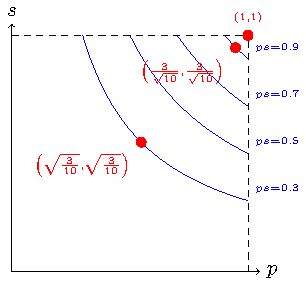
\includegraphics{images/original_space.pdf}}\qquad
	\subfloat[The transformed space for the $k$ nearest neighbours problem.]{\label{fig:knnspace}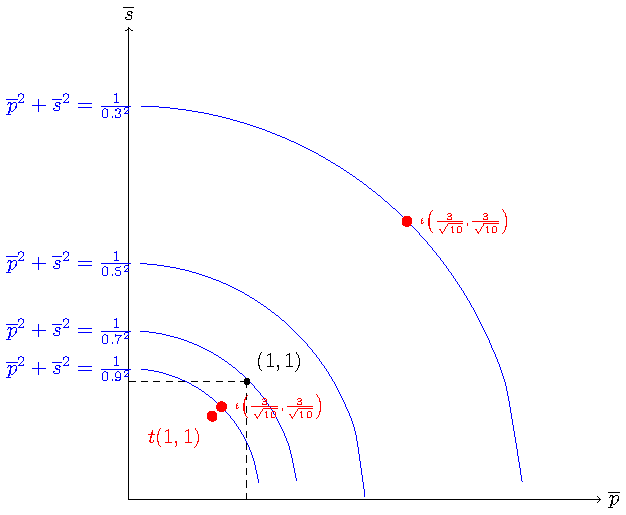
\includegraphics[scale=0.55]{images/transformed_space.pdf}}\\
	\caption{Two different characterizations of the probabilistic trace alignment problem. The best possible match is represented in red in both the similarity/probability space and in the transformed one.}
\end{figure}


 We can show with the next lemma that the following transformation is the one reducing the problem to the $k$-Nearest Neighbour problem:



\begin{lemma}
Given a value $k\in[0,1]\subseteq \mathbb{R}^+_0$, the set of points having the product $ps$ at least $k$ corresponts to the set of $t$-transformed points having a distance of at least $1/k$ from the origin of the axes.
\end{lemma}
\begin{proof}
\[\begin{aligned}
ps\geq k&\Leftrightarrow \frac{1}{ps}\leq\frac{1}{k} \\
	   &\Leftrightarrow \frac{\sqrt{p^2+s^2}}{ps\sqrt{p^2+s^2}}\leq\frac{1}{k} \\
	   &\Leftrightarrow \sqrt{\frac{p^2+s^2}{p^2s^2(p^2+s^2)}}\leq\frac{1}{k} \\
	   &\Leftrightarrow \sqrt{\frac{p^2}{p^2s^2(p^2+s^2)}+\frac{s^2}{p^2s^2(p^2+s^2)}}\leq\frac{1}{k} \\
	   &\Leftrightarrow \sqrt{\frac{1}{s^2(p^2+s^2)}+\frac{1}{p^2(p^2+s^2)}}\leq\frac{1}{k} \\
	   &\Leftrightarrow \left\|{\biggr({\frac{1}{s\sqrt{p^2+s^2}},\frac{1}{p\sqrt{p^2+s^2}}\biggr)}-\vec{0}}\right\|_2\leq\frac{1}{k} \\
	   &\Leftrightarrow \left\|t(p,s)-\vec{0}\right\|_2\leq\frac{1}{k} \\
\end{aligned}\]
\end{proof}
\begin{lemma}
Given a Petri Net $P$ and a trace $t^*$, the probabilistic trace alignment problem of the best $k$ traces reduces to the $k$-Nearest Neighbour problem $\mu_{\tau^*}^{-1}(knn(k,\vec{0},\mu_{\tau^*}(\mathcal{W}_0^{\aleph_0}(P))))$.
\end{lemma}
\begin{proof}
Trivial by definition of $\mu_{\tau^*}$ and for the previous lemma.
\end{proof}

\begin{table}[!t]
\centering
\caption{Representing the point from Table \ref{tab:expected} in the transformed space.}\label{tab:transf}
\begin{tabular}{ll|lll}
	\toprule
	
	$\tau$ & $t(\mu_{\tau^*}(\tau))$ & $\norm{t(\mu_{\tau^*}(\tau))-\vec{0}}{2}$ & $\frac{1}{\norm{t(\mu_{\tau^*}(\tau))-\vec{0}}{2}}$ & \textit{distance ranking}\\
	
	\midrule	
	a   & $\braket{2.16, \;\,3.37}$ & $4.00$ & $0.2500$ & \textbf{1}\\
	{aa}  & $\braket{1.89, \;\,6.74}$ & $7.00$ & $0.1428$ & \textbf{2}\\
	aaa   & $\braket{1.94, 13.87}$ & $14.00$ & $0.0714$ & \textbf{3}\\
	ca   & $\braket{1.95, 19.91}$ & $20$ & $0.0500$ & \textbf{4}\\
	{cb}  & $\braket{1.95, 23.25}$ & $23.33$ & $0.0428$ & \textbf{5}\\
aaaa   & $\braket{1.95, 27.93}$ & $28.00$ & $0.0357$ & \textbf{6}\\
caa   & $\braket{1.44, 34.26}$ & $34.29$ & $0.0292$ & \textbf{7}\\
caaa   & $\braket{1.44, 68.56}$ & $68.57$ & $0.0145$ & \textbf{8}\\
	\bottomrule
\end{tabular}
\end{table}
\begin{example}
We now want to show the correctness of the former lemmas with some examples.
Table \ref{tab:transf} represents the transformed points $t(\mu_{\tau^*}(\tau))$ from the data points $\mu_{\tau^*}(\tau)$  calculated  Example \ref{ex:rankingTaus}. The third column shows the distance of the transformed point from the origin: the following column shows that the inverse of such distance exactly represents the previously calculated $s_d(\tau,\tau^*)\cdot w_\tau$, thus empirically implying that the $k$-nearest neighbours problem corresponts to the best $k$ traces maximising the product $s_d(\tau,\tau^*)\cdot w_\tau$.
\end{example}





At this stage, we can solve the $k$-probabilistic trace alignment problem by generating a new instance of the $k$-Nearest Neighbour problem for each possible trace $\tau^*$ that we want to align towards the traces coming from a TG. On the other hand, this solution might result quite costly, as solving the problem would require either to use a brute force search algorithm or to load and index our set of points each time.\yellownote{TODO: add references and explanation to the problem (we need a Related Work section\dots? I am accustomed to write such sections.)} In the next section we will discuss an approximated version of the problem providing a trade-off between accuracy and efficiency.


\subsection{Approximate $k$-probabilistic Traces Alignment Problem}\label{subsec:akptap}
Given that in the approximated characterization the traces are immediately represented as vectors, we can observe that the approximate $k$-probabilistic Trace Alignment Problem can be characterized as $knn_d(k,\phi(\tau^*),\phi(\mathcal{W}_{p_\theta}(P)))$, where $d(u,v)$ is defined as the inverse of the normalized dot product, i.e. $d(u,v)=1-\frac{\braket{u,v}}{\sqrt{\braket{u,u}\braket{v,v}}}$. 



\textit{Trace alignments algorithms provide as output a single alignment. This is not very convenient in practice because a rich feedback should provide different possibilities. This is even more important when the Petri Net we are considering is stochastic and the different model traces have different probabilities.}

\textit{INPUT: trace, stochastic (Workflow net) Petri Net, minimum probability threshold, maximum model trace length
OUTPUT: set of model traces satisfying the minimum probability threshold and the maximum model trace length candidates for the alignment with an alignment ranking}
